% fig2_model.tex -- footprints, multiplicity, the nerve and the k-fold region,
% and what they say about an onset zone.  Six contacts on a ring of radius
% 1.4 with footprints of radius 1 (top row); the same with one contact added
% at the centre (bottom row).  Every statement in the panel titles was
% checked numerically (exact enclosing-circle tests for the nerve, and a
% 1501^2 raster for the Betti numbers of R_1 and R_2).
\documentclass[tikz,border=4pt]{standalone}
% ecogstyle.tex -- colours, fonts and plot defaults shared by every figure of
% ecog_coverage.tex.  \input by each standalone figure in this directory.
%
% Colour roles (validated as one categorical palette: adjacent and all-pairs
% CVD separation >= 9, normal-vision separation >= 16; aqua sits below 3:1
% against white, so every aqua mark also carries a marker and a direct label):
%   cBlue    contacts placed by covering radius, single coverage (k = 1)
%   cOrange  the documented 8x8 subdural grid
%   cAqua    contacts restricted to gyral crowns (what a sheet can reach)
%   cViolet  contacts placed by covering radius, double coverage (k = 2)
%   cRed     cortex no contact sees; an onset zone that is missed
\usepackage{amsmath,amssymb}
\usepackage{lmodern}
\usepackage[T1]{fontenc}
\usepackage{tikz}
\usepackage{pgfplots}
\pgfplotsset{compat=1.18}
\usetikzlibrary{arrows.meta,positioning,shapes.geometric,shapes.misc,
  calc,fit,backgrounds,decorations.pathreplacing,patterns,shadows}
\usepgfplotslibrary{fillbetween,groupplots}

\definecolor{cBlue}{HTML}{2A78D6}
\definecolor{cOrange}{HTML}{EB6834}
\definecolor{cAqua}{HTML}{1BAF7A}
\definecolor{cViolet}{HTML}{4A3AA7}
\definecolor{cRed}{HTML}{E34948}
\definecolor{cInk}{HTML}{0B0B0B}
\definecolor{cInk2}{HTML}{52514E}
\definecolor{cMuted}{HTML}{8A8983}
\definecolor{cGrid}{HTML}{E4E3DF}
\definecolor{cSurface}{HTML}{FCFCFB}
\definecolor{cWash}{HTML}{F3F2EF}
\definecolor{cCortex}{HTML}{D9CFC4}
\definecolor{cCortexDark}{HTML}{9C8B7A}
\definecolor{cBlueLight}{HTML}{CDE2FB}
\definecolor{cBlueMid}{HTML}{86B6EF}

\pgfplotsset{
  ecog/.style={
    width=7.2cm, height=5.4cm,
    axis line style={cInk2, line width=0.5pt},
    tick style={cInk2, line width=0.5pt},
    major tick length=3pt,
    grid=major,
    grid style={cGrid, line width=0.4pt, solid},
    tick label style={font=\footnotesize, text=cInk2},
    label style={font=\small, text=cInk},
    title style={font=\small\bfseries, text=cInk, align=center},
    legend style={font=\footnotesize, draw=none, fill=white,
      fill opacity=0.9, text opacity=1, text=cInk,
      row sep=1pt, inner sep=2pt},
    legend cell align=left,
    every axis plot/.append style={line width=1.4pt, line join=round,
      line cap=round},
    axis background/.style={fill=white},
    clip marker paths=true,
  },
  mk/.style={mark=*, mark size=2.1pt,
    mark options={solid, draw=white, line width=0.6pt}},
  mksq/.style={mark=square*, mark size=2.0pt,
    mark options={solid, draw=white, line width=0.6pt}},
  mktri/.style={mark=triangle*, mark size=2.6pt,
    mark options={solid, draw=white, line width=0.6pt}},
  mkdia/.style={mark=diamond*, mark size=2.7pt,
    mark options={solid, draw=white, line width=0.6pt}},
}

% panel letters
\newcommand{\panel}[1]{\textbf{\sffamily (#1)}}
\tikzset{
  panellabel/.style={font=\small\bfseries\sffamily, text=cInk,
    anchor=north west, inner sep=0pt},
  note/.style={font=\footnotesize, text=cInk2, align=center},
}

\begin{document}
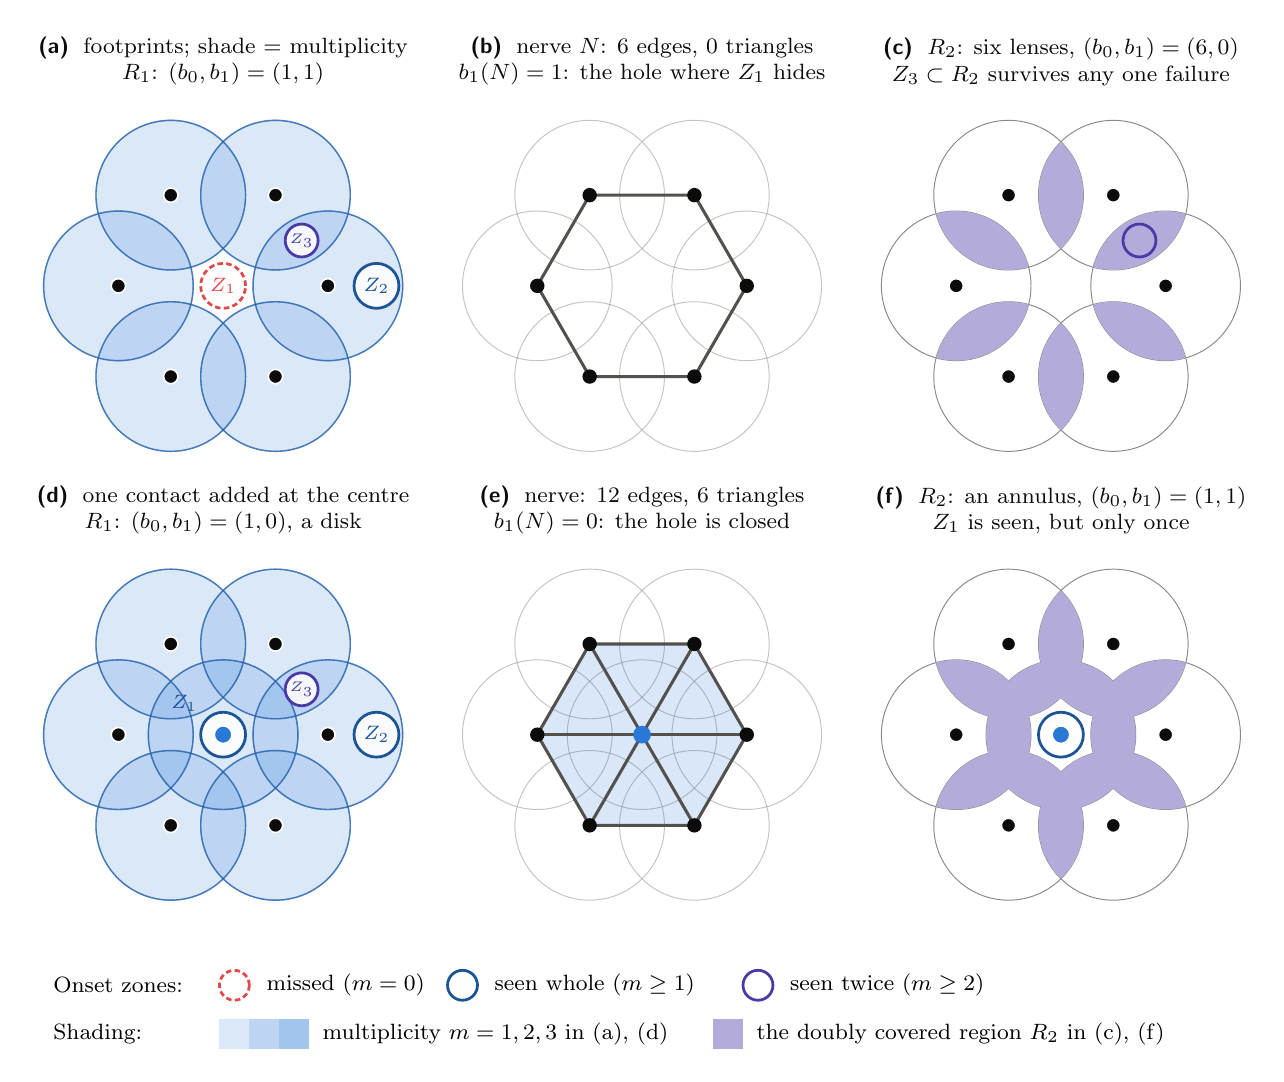
\begin{tikzpicture}[
  x=0.95cm, y=0.95cm,
  contact/.style={circle, fill=cInk, draw=white, line width=0.6pt,
    inner sep=0pt, minimum size=5.2pt},
  newcontact/.style={contact, fill=cBlue, minimum size=6.4pt},
  fp/.style={fill=cBlue, fill opacity=0.17, draw=cBlue!80!black,
    draw opacity=0.55, line width=0.5pt},
  zone/.style={line width=1.0pt, fill=white, fill opacity=0.85},
  zmiss/.style={zone, draw=cRed, dash pattern=on 2pt off 1.2pt},
  zonce/.style={zone, draw=cBlue!70!black},
  ztwice/.style={zone, draw=cViolet},
  zlab/.style={font=\scriptsize\itshape, inner sep=1pt},
  nv/.style={circle, fill=cInk, inner sep=0pt, minimum size=5.2pt},
  ne/.style={line width=1.1pt, cInk2},
  ptitle/.style={font=\footnotesize, text=cInk, align=center, anchor=south},
]
\def\ring{1.4}
% contact coordinates and onset-zone centres, defined inside each panel so
% that they move with its shift; radii in units of the footprint radius
\newcommand{\defcoords}{%
  \foreach \i in {0,...,5} {\coordinate (c\i) at ({60*\i}:\ring);}%
  \coordinate (c6) at (0,0);%
  \coordinate (zm) at (0,0);%
  \coordinate (zo) at (2.05,0);%
  \coordinate (zt) at (30:1.2124);}
\def\rm{0.30}\def\ro{0.30}\def\rt{0.22}

% ======================================================= row 1: the ring
% (a) footprints and multiplicity
\begin{scope}[shift={(0,0)}]
  \defcoords
  \foreach \i in {0,...,5} {\fill[fp] (c\i) circle (1);}
  \foreach \i in {0,...,5} {\draw[cBlue!80!black, line width=0.5pt, opacity=0.6] (c\i) circle (1);}
  \draw[zmiss] (zm) circle (\rm);
  \draw[zonce] (zo) circle (\ro);
  \draw[ztwice] (zt) circle (\rt);
  \foreach \i in {0,...,5} {\node[contact] at (c\i) {};}
  \node[zlab, text=cRed] at (0,0) {$Z_1$};
  \node[zlab, text=cBlue!70!black] at (zo) {$Z_2$};
  \node[zlab, text=cViolet, font=\tiny\itshape] at (zt) {$Z_3$};
  \node[ptitle] at (0,2.55) {\panel{a}\; footprints; shade $=$ multiplicity\\
    $R_1$: $(b_0,b_1)=(1,1)$};
\end{scope}
% (b) the nerve
\begin{scope}[shift={(5.6,0)}]
  \defcoords
  \foreach \i in {0,...,5} {\draw[cMuted, line width=0.35pt, opacity=0.5] (c\i) circle (1);}
  \draw[ne] (c0)--(c1)--(c2)--(c3)--(c4)--(c5)--cycle;
  \foreach \i in {0,...,5} {\node[nv] at (c\i) {};}
  \node[ptitle] at (0,2.55) {\panel{b}\; nerve $N$: 6 edges, 0 triangles\\
    $b_1(N)=1$: the hole where $Z_1$ hides};
\end{scope}
% (c) the doubly covered region
\begin{scope}[shift={(11.2,0)}]
  \defcoords
  \foreach \i in {0,...,5} {\draw[cMuted, line width=0.35pt] (c\i) circle (1);}
  \foreach \i/\j in {0/1,1/2,2/3,3/4,4/5,5/0} {
    \begin{scope}\clip (c\i) circle (1); \fill[cViolet!42] (c\j) circle (1);\end{scope}}
  \draw[ztwice, fill opacity=0] (zt) circle (\rt);
  \foreach \i in {0,...,5} {\node[contact] at (c\i) {};}
  \node[ptitle] at (0,2.55) {\panel{c}\; $R_2$: six lenses, $(b_0,b_1)=(6,0)$\\
    $Z_3\subset R_2$ survives any one failure};
\end{scope}

% ================================================ row 2: one contact added
\begin{scope}[shift={(0,-6.0)}]
  \defcoords
  \foreach \i in {0,...,6} {\fill[fp] (c\i) circle (1);}
  \foreach \i in {0,...,6} {\draw[cBlue!80!black, line width=0.5pt, opacity=0.6] (c\i) circle (1);}
  \draw[zonce] (zm) circle (\rm);
  \draw[zonce] (zo) circle (\ro);
  \draw[ztwice] (zt) circle (\rt);
  \foreach \i in {0,...,5} {\node[contact] at (c\i) {};}
  \node[newcontact] at (c6) {};
  \node[zlab, text=cBlue!70!black] at (-0.52,0.42) {$Z_1$};
  \node[zlab, text=cBlue!70!black] at (zo) {$Z_2$};
  \node[zlab, text=cViolet, font=\tiny\itshape] at (zt) {$Z_3$};
  \node[ptitle] at (0,2.55) {\panel{d}\; one contact added at the centre\\
    $R_1$: $(b_0,b_1)=(1,0)$, a disk};
\end{scope}
\begin{scope}[shift={(5.6,-6.0)}]
  \defcoords
  \foreach \i in {0,...,6} {\draw[cMuted, line width=0.35pt, opacity=0.5] (c\i) circle (1);}
  \foreach \i/\j in {0/1,1/2,2/3,3/4,4/5,5/0} {\fill[cBlue, fill opacity=0.18] (c6)--(c\i)--(c\j)--cycle;}
  \draw[ne] (c0)--(c1)--(c2)--(c3)--(c4)--(c5)--cycle;
  \foreach \i in {0,...,5} {\draw[ne] (c6)--(c\i);}
  \foreach \i in {0,...,5} {\node[nv] at (c\i) {};}
  \node[nv, fill=cBlue, minimum size=6.4pt] at (c6) {};
  \node[ptitle] at (0,2.55) {\panel{e}\; nerve: 12 edges, 6 triangles\\
    $b_1(N)=0$: the hole is closed};
\end{scope}
\begin{scope}[shift={(11.2,-6.0)}]
  \defcoords
  \foreach \i in {0,...,6} {\draw[cMuted, line width=0.35pt] (c\i) circle (1);}
  \foreach \i/\j in {0/1,1/2,2/3,3/4,4/5,5/0,0/6,1/6,2/6,3/6,4/6,5/6} {
    \begin{scope}\clip (c\i) circle (1); \fill[cViolet!42] (c\j) circle (1);\end{scope}}
  \draw[zonce, fill opacity=0] (zm) circle (\rm);
  \foreach \i in {0,...,5} {\node[contact] at (c\i) {};}
  \node[newcontact] at (c6) {};
  \node[ptitle] at (0,2.55) {\panel{f}\; $R_2$: an annulus, $(b_0,b_1)=(1,1)$\\
    $Z_1$ is seen, but only once};
\end{scope}

% ================================================================ legend
\begin{scope}[shift={(-2.4,-9.35)}]
  \node[anchor=west, font=\footnotesize] at (0,0) {Onset zones:};
  \draw[zmiss, fill opacity=0] (2.55,0) circle (0.2);
  \node[anchor=west, font=\footnotesize] at (2.85,0) {missed ($m=0$)};
  \draw[zonce, fill opacity=0] (5.6,0) circle (0.2);
  \node[anchor=west, font=\footnotesize] at (5.9,0) {seen whole ($m\ge1$)};
  \draw[ztwice, fill opacity=0] (9.55,0) circle (0.2);
  \node[anchor=west, font=\footnotesize] at (9.85,0) {seen twice ($m\ge2$)};
  \node[anchor=west, font=\footnotesize] at (0,-0.65) {Shading:};
  \fill[cBlue, fill opacity=0.17] (2.35,-0.85) rectangle ++(0.4,0.4);
  \fill[cBlue, fill opacity=0.31] (2.75,-0.85) rectangle ++(0.4,0.4);
  \fill[cBlue, fill opacity=0.43] (3.15,-0.85) rectangle ++(0.4,0.4);
  \node[anchor=west, font=\footnotesize] at (3.6,-0.65) {multiplicity $m=1,2,3$ in (a), (d)};
  \fill[cViolet!42] (8.95,-0.85) rectangle ++(0.4,0.4);
  \node[anchor=west, font=\footnotesize] at (9.4,-0.65) {the doubly covered region $R_2$ in (c), (f)};
\end{scope}
\end{tikzpicture}
\end{document}
